\begin{figure}[H]
    \centering
    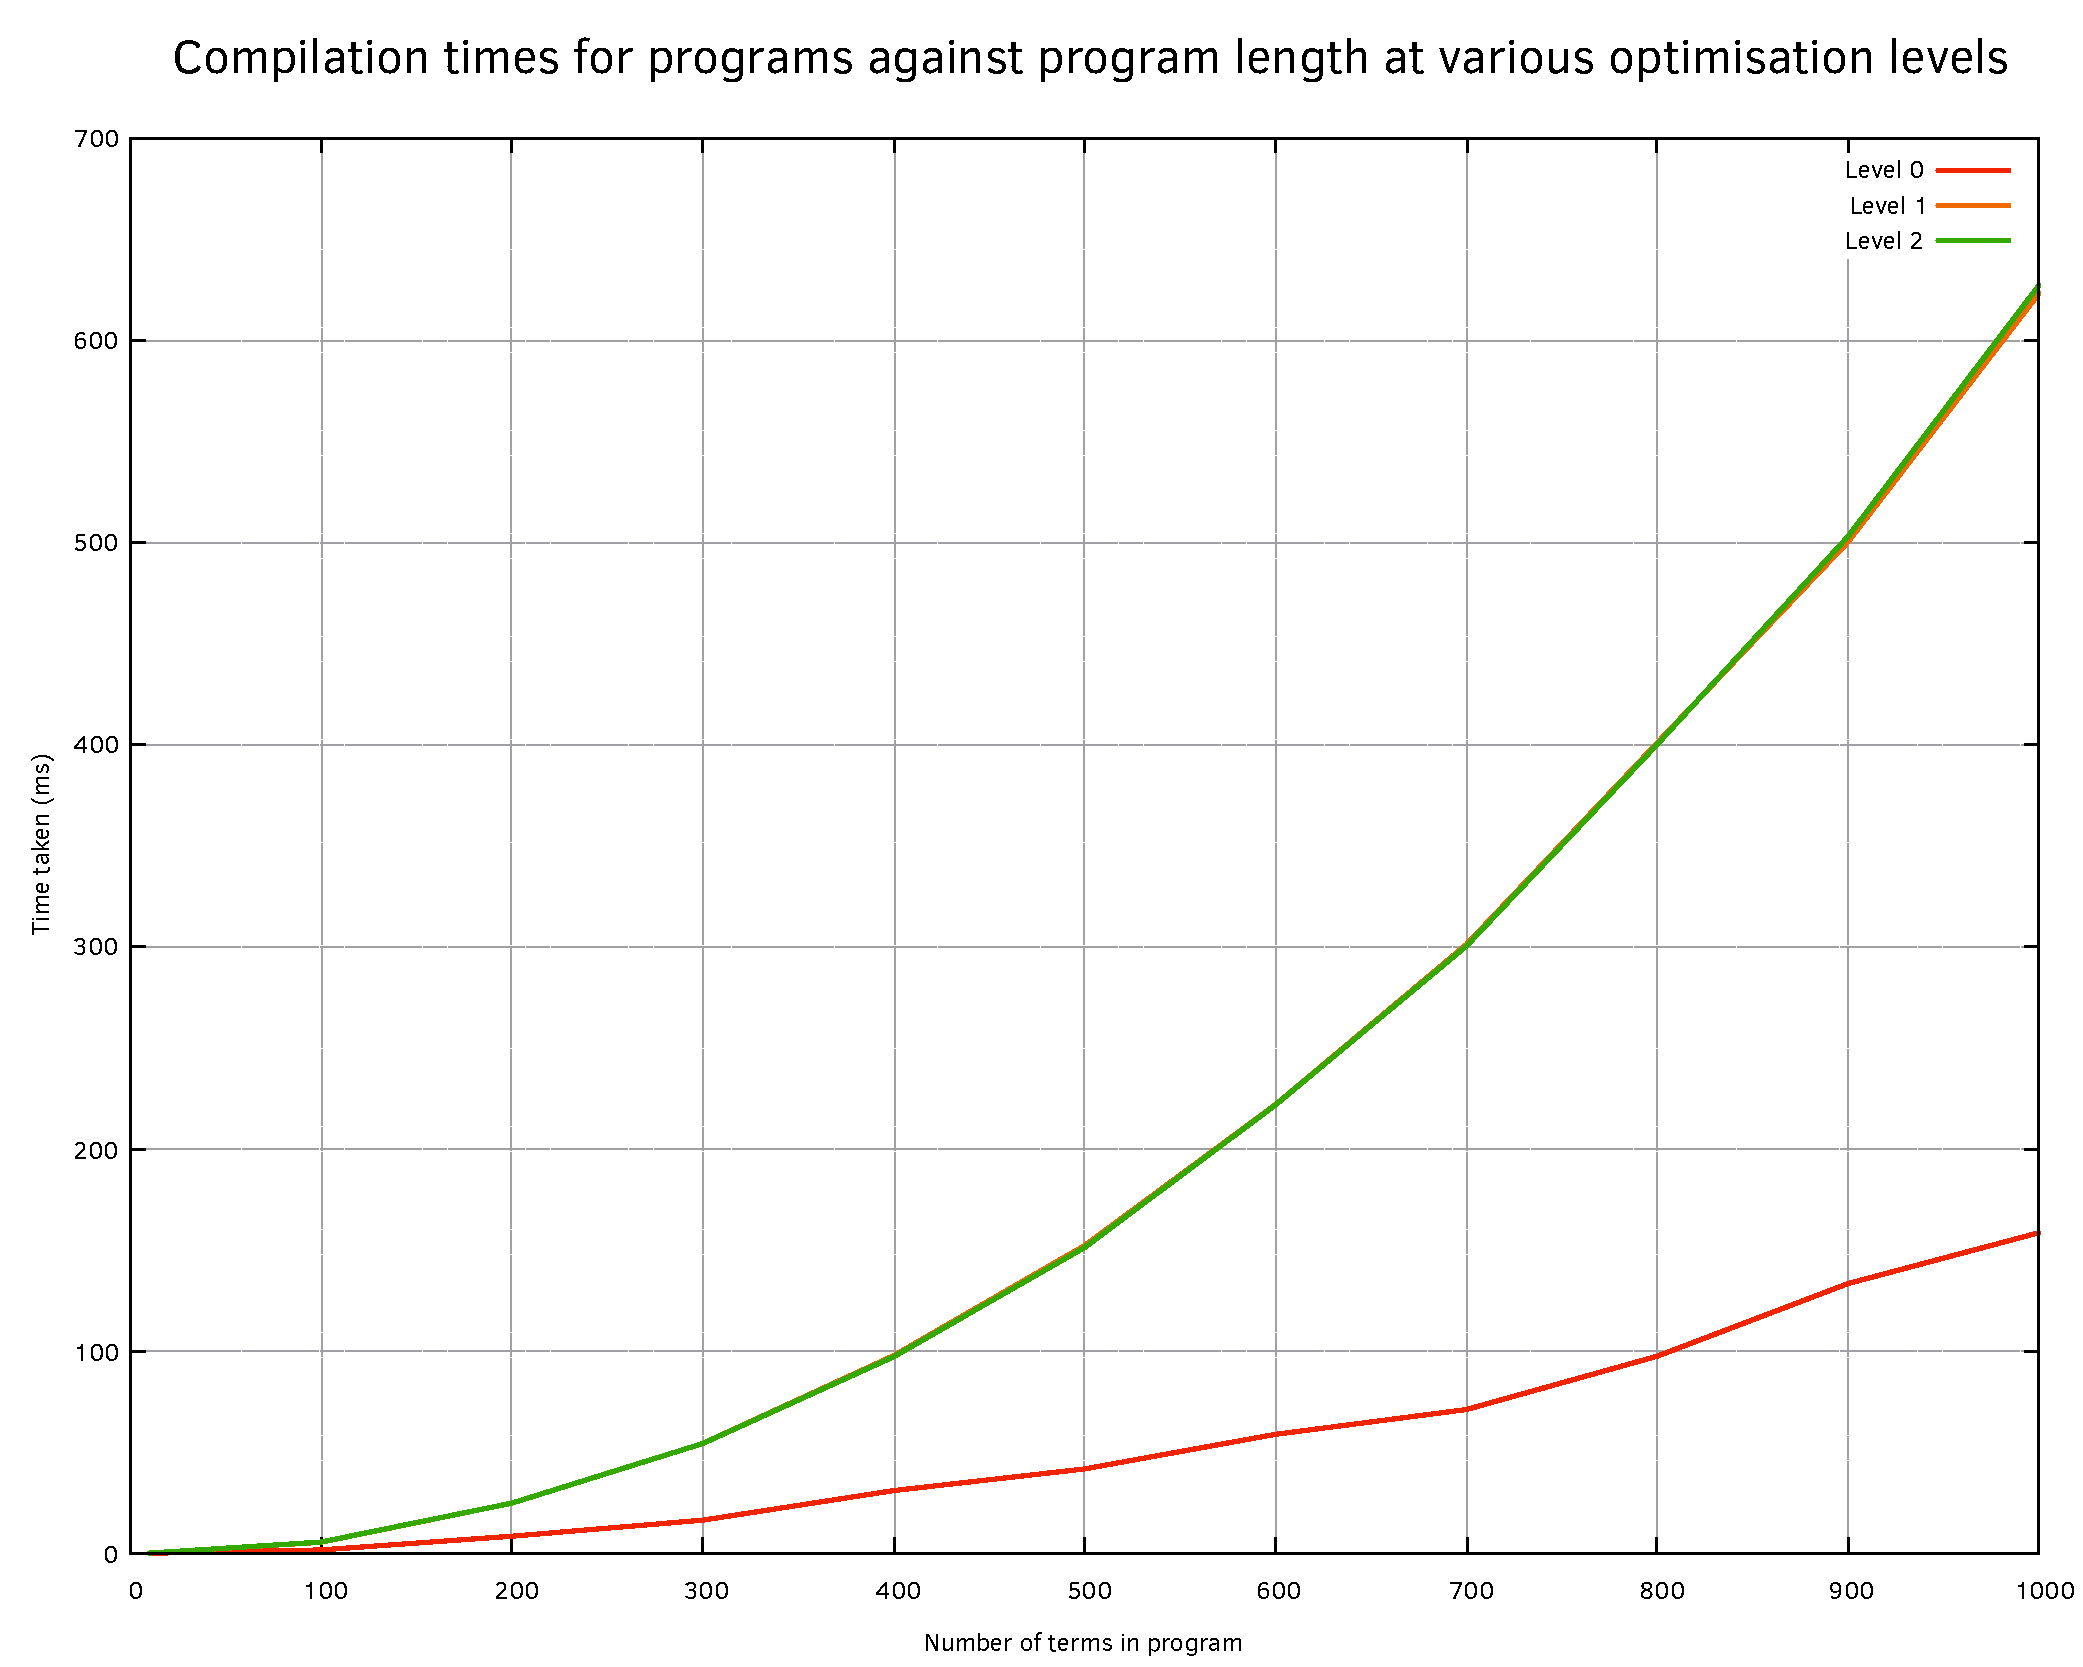
\includegraphics[width=\textwidth - 100pt]{04_results/images/compilation_results}

    \begin{center}
    \begin{tabular}{ |c|c|c|c|c| } 
    \hline
    Program & Program Length & Level 0 & Level 1 & Level 2 \\ 
    \hline
    delve & 10 & 14.365 us & 55.416 us & 60.233 us\\
    \hline
    delve & 100 & 1.6734 ms & 5.4487 ms & 5.5868 ms\\
    \hline
    delve & 200 & 8.3995 ms & 24.780 ms & 24.802 ms\\
    \hline
    delve & 300 & 16.349 ms	& 54.290 ms& 54.245 ms\\
    \hline
    delve & 400 & 30.992 ms & 97.726 ms & 	97.198 ms\\
    \hline
    delve & 500 & 41.730 ms &152.20 ms & 151.23 ms \\
    \hline
    delve & 600 & 58.856 ms &221.79 ms & 221.72 ms \\
    \hline
    delve & 700 & 71.066 ms &300.98 ms & 300.28 ms \\
    \hline
    delve & 800 & 97.426 ms &400.76 ms & 399.97 ms \\
    \hline
    delve & 900 & 133.36 ms &500.20 ms & 502.94 ms \\
    \hline
    delve & 1000 & 158.58 ms & 623.05 ms & 627.05 ms \\
    \hline
    \end{tabular}
    \end{center}
    \caption{Program length vs compilation time at various optimisation levels.}
    \label{fig:compilation_results}
\end{figure}
